%----------------------------------------------------------------------------------------
%	PACKAGES AND DOCUMENT CONFIGURATIONS
%----------------------------------------------------------------------------------------
\documentclass{article}

\usepackage[utf8]{inputenc}
\usepackage[T1]{fontenc}
\usepackage[brazilian]{babel}
\usepackage{graphicx}
\usepackage[a4paper, margin=4cm]{geometry}
\usepackage{url}
\usepackage{indentfirst}
\usepackage{mathtools}
\usepackage{listings}
\usepackage[toc,page]{appendix}
\usepackage{color}

\setlength{\parindent}{4em}
\setlength{\parskip}{0.5em}

\definecolor{commentgreen}{rgb}{0,0.5,0}

\lstset{breaklines=true,
  basicstyle=\footnotesize,
  frame=single,
  keepspaces=true,
  numberstyle=\tiny\color{gray},
  language=C++,
  keywordstyle=\color{blue},
  commentstyle=\color{commentgreen},
  stringstyle=\color{red},
  extendedchars=false,
  showstringspaces=false,
  literate=
  {á}{{\'a}}1 {é}{{\'e}}1 {í}{{\'i}}1 {ó}{{\'o}}1 {ú}{{\'u}}1
  {Á}{{\'A}}1 {É}{{\'E}}1 {Í}{{\'I}}1 {Ó}{{\'O}}1 {Ú}{{\'U}}1
  {à}{{\`a}}1 {è}{{\`e}}1 {ì}{{\`i}}1 {ò}{{\`o}}1 {ù}{{\`u}}1
  {À}{{\`A}}1 {È}{{\'E}}1 {Ì}{{\`I}}1 {Ò}{{\`O}}1 {Ù}{{\`U}}1
  {ä}{{\"a}}1 {ë}{{\"e}}1 {ï}{{\"i}}1 {ö}{{\"o}}1 {ü}{{\"u}}1
  {Ä}{{\"A}}1 {Ë}{{\"E}}1 {Ï}{{\"I}}1 {Ö}{{\"O}}1 {Ü}{{\"U}}1
  {â}{{\^a}}1 {ê}{{\^e}}1 {î}{{\^i}}1 {ô}{{\^o}}1 {û}{{\^u}}1
  {Â}{{\^A}}1 {Ê}{{\^E}}1 {Î}{{\^I}}1 {Ô}{{\^O}}1 {Û}{{\^U}}1
  {œ}{{\oe}}1 {Œ}{{\OE}}1 {æ}{{\ae}}1 {Æ}{{\AE}}1 {ß}{{\ss}}1
  {ű}{{\H{u}}}1 {Ű}{{\H{U}}}1 {ő}{{\H{o}}}1 {Ő}{{\H{O}}}1
  {ç}{{\c c}}1 {Ç}{{\c C}}1 {ø}{{\o}}1 {å}{{\r a}}1 {Å}{{\r A}}1
  {€}{{\EUR}}1 {£}{{\pounds}}1,
}

%\setlength\parindent{0pt} % Removes all indentation from paragraphs

%----------------------------------------------------------------------------------------
%	DOCUMENT INFORMATION
%----------------------------------------------------------------------------------------

\title{Um Modelo Matemático para Análise de Batalhas Históricas Considerando Munição Limitada} % Title

\author{Thales Luis Rodrigues Sabino} % Author name

\date{\today} % Date for the report

\begin{document}

\maketitle % Insert the title, author and date

\begin{center}
Relatório técnico do trabalho realizado na disciplina \textit{Instrução a Modelagem Matemática (2015-3)} do \textbf{Programa de Pós-Graduação em Modelagem Computacional (PGMC)} \textbf{da Universidade Federal de Juiz de Fora (UFJF)}.
\end{center}


\begin{center}
\textbf{Professor:} Rodrigo Weber dos Santos
\end{center}

% If you wish to include an abstract, uncomment the lines below
\begin{abstract}
Abstract text
\end{abstract}

%----------------------------------------------------------------------------------------
%	SECTION 1
%----------------------------------------------------------------------------------------

\section{Introdução}

Descoberta no século 19 na antiga Suméria, a cidade-estado de Lagash possui ruínas que contém registros que mostram vários aspectos da guerra travada com uma cidade-estado vizinha conhecida como Umma. Nas ruínas foram encontradas representações de soldados sendo devorados por abutres. A relíquia, hoje, encontra-se exposta no Museu do Louvre, em Paris \cite{firstwar}.

Fica claro que conflitos, armados ou não, sempre fizeram parte da história da humanidade. O orçamento dedicado a defesa de vários países corresponde a uma parte significativa do PIB gerado, tornando o aspecto bélico de extrema importância para a defesa e segurança de um país (procurar referência).

É evidente que uma parte significa do dinheiro investido nas forças militares é dedicada ao estudo de situações de combate, estratégias e maneiras eficientes de vencer as batalhas. O termo eficiente, nesse contexto, significa derrotar o inimigo sofrendo um número mínimo de baixas. 

Não faz parte do escopo deste trabalho a realização de uma discussão sobre os aspectos positivos, negativos e impactos sociais causados por conflitos, somente uma análise de um modelo  matemático que tenta capturar os aspectos de um conflito armado entre dois exércitos homogêneos.

\subsection{Modelos de Combate do Tipo Lanchester}

A análise de combates do ponto de vista matemático foi inicialmente desenvolvido por Frederick W. Lanchester (1914) (Figura \ref{fig:fw-lanchester}), um engenheiro britânico que que desenvolveu a teoria dos combates baseado em conflitos aéreos da Primeira Guerra Mundial na tentativa de explicar porque a concentração de forças era útil em combates modernos. As \textit{leis} de Lanchester são ensinadas e usadas em todos os colégios militares do mundo.

\begin{figure}[ht]
	\centering
	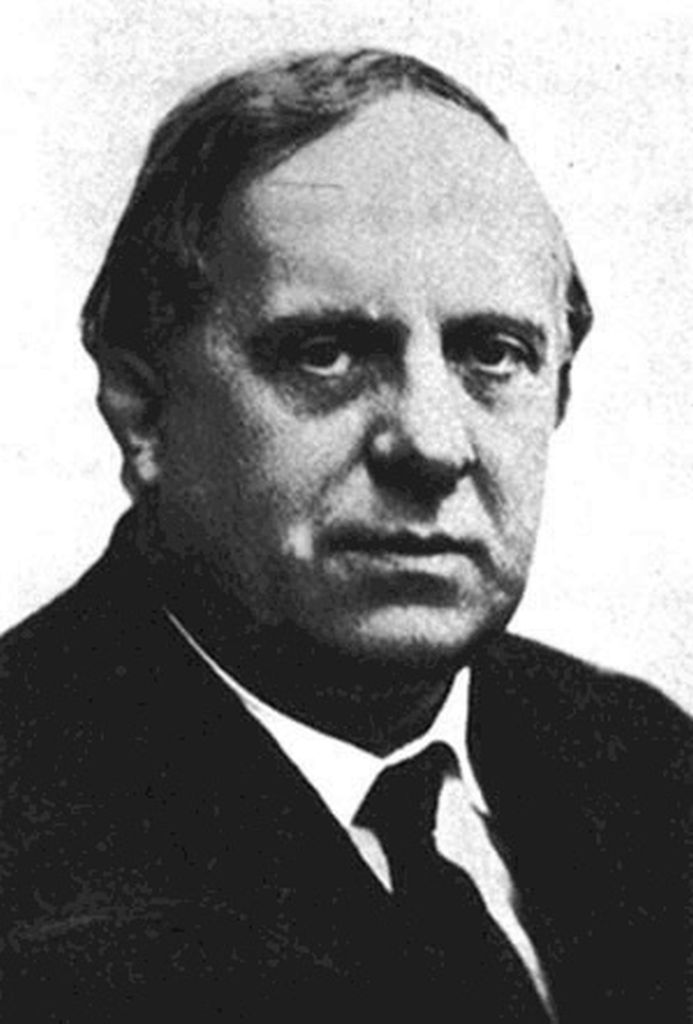
\includegraphics[width=0.3\linewidth]{figs/fw_lanchester_693x1024.jpg}
	\caption{Frederick Willian Lanchester}
	\label{fig:fw-lanchester}
\end{figure}

Existem dois tipos de modelos a serem considerados, \textbf{homogêneos} e \textbf{heterogêneos}. No modelo homogêneo, um único escalar é utilizado para representar o poder de combate de uma unidade e ambos os lados do conflito são considerados equivalentes quanto a eficiência em combate. O modelo homogêneo pode ser considerado de cunho \textit{acadêmico} e é aplicado na análise e revisão de \textit{batalhas históricos}, não sendo considerado um bom modelo para descrição de \textit{combates modernos} \cite{giordana03first}.

\subsection{Batalhas Históricas}

Não foi considerada nenhuma batalha específica no desenvolvimento deste trabalho, somente a forma como as batalhas eram efetuadas.

Antes da Primeira Guerra Mundial, conhecida como guerra das trincheiras, as batalhas entre dois países que estavam em guerra tinham um formato bem diferente dos combates modernos. As batalhas, normalmente, tinham um local e data pré-definidos, onde das duas forças se encontravam e faziam a disputa. A força que conseguisse incapacitar a maior parte da força do adversário era considerada a vencedora. Nesse tipo de conflito, os dois exércitos praticamente se alinhavam um de frente para o outro, em uma formação, normalmente em linha ou retangular até que fosse ordenado o ataque. A linha de frente de cada exército ia sendo substituída a medida que os soldados iam ficando sem munição ou era atingidos. 

A \textbf{Batalha de Gettysburg} (Figura \ref{fig:gettysburg-battle}) é uma batalha famosa da Guerra Civil Americana conhecida por ser a batalha com maior número de vítimas de tal guerra. O \textbf{Assalto de Pickett} (\ref{fig:picketts-charge}) foi o famoso assalto da infantaria Confederada ordenada pelo Gal. Robert E. Lee, em 3 de Julho de 1863, durante a Batalha de Gettsburg. No entanto, esse assalto foi repelido com um grande número de baixas e decisão a favor da União.

\begin{figure}[ht]
	\centering
	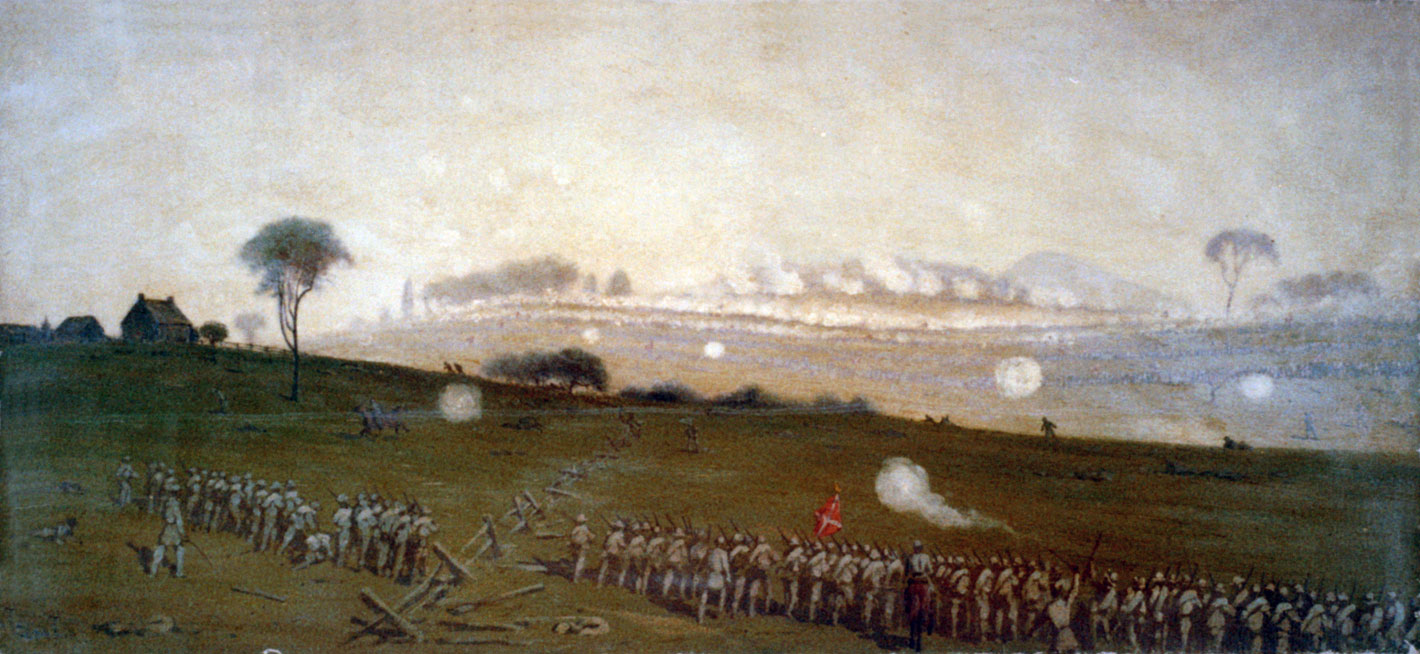
\includegraphics[width=0.9\linewidth]{figs/edwin_forbes_picketts_charge_1420x654.jpg}
	\caption{O Assalto de Pickett de uma posição na linha dos Confederados olhando para as linhas da União. Pintura de Edwin Forbes.}
	\label{fig:picketts-charge}
\end{figure}

\begin{figure}[ht]
	\centering
	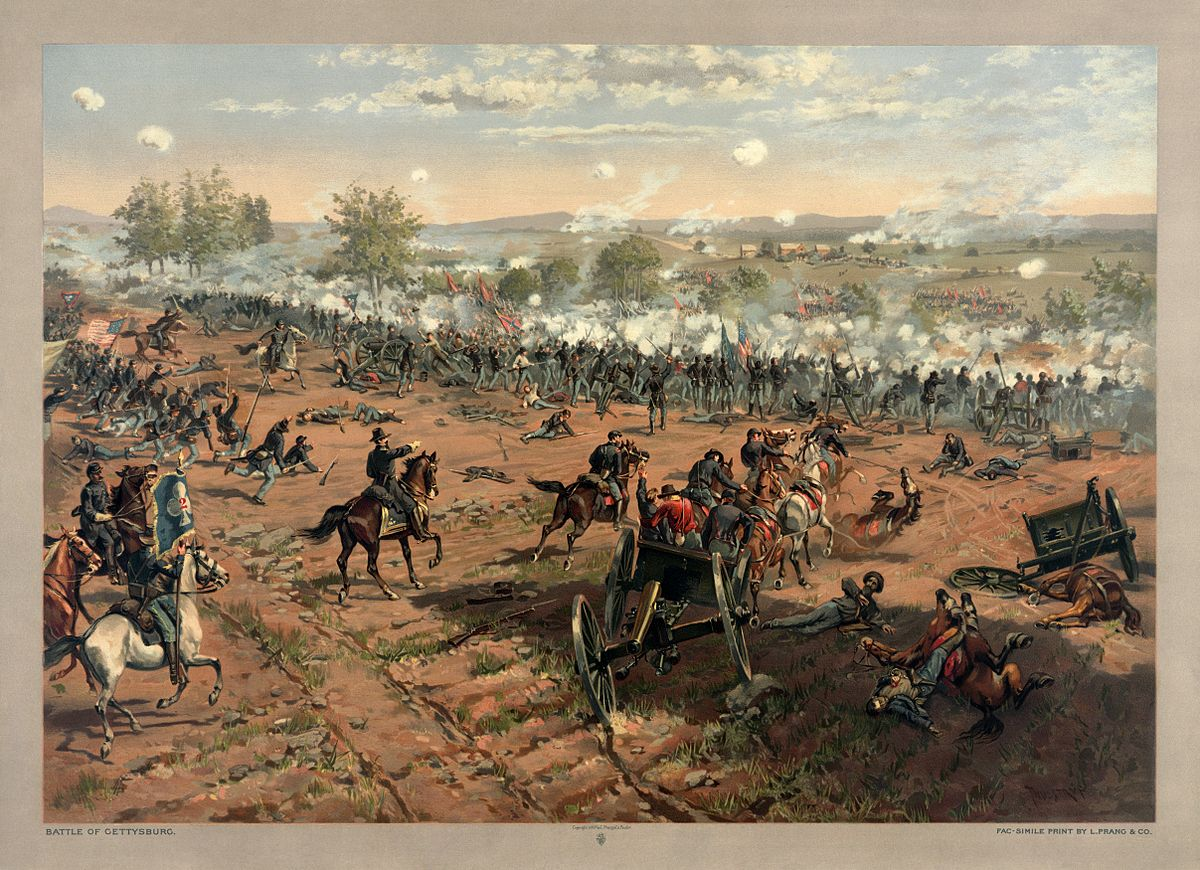
\includegraphics[width=0.7\linewidth]{figs/Battle_of_Gettysburg_1200x870.jpg}
	\caption{Pintura da Batalha de Gettysburg}
	\label{fig:gettysburg-battle}	
\end{figure}

As \textbf{Equações de Lanchester} foram utilizas para modelar esse conflito e, portanto, representam um modelo válido para o estudo de conflitos clássicos.

O modelo matemático apresentado neste trabalho foi ligeiramente baseado no modelo de forças homogêneas de Lanchester, porém foi considerado que a munição disponível na linha de frente é limitada e deve ser reposta. Para modelar a reposição da munição na linha de frente foi utilizado o processo de difusão, onde a munição deve sair da retaguarda até chegar na linha de frente onde pode ser utilizada contra o exército inimigo.

\section{Objetivo}

O objetivo deste trabalho é o desenvolvimento e análise de um modelo matemático capaz de representar o embate entre duas forças homogêneas, porém com munição disponível limitada na linha de frente. 

O modelo proposto foi baseado no modelo de Lanchester porém foram acrescentados outros parâmetros de forma a a permitir um controle mais refinado do desenrolar da batalha. 

\section{Modelo Matemático de Batalhas Históricas}

Considere o embate entre duas forças homogêneas no contexto de uma batalha histórica, onde os exércitos se alinham um de frente para o outro em formação e mantém a posição atirando e substituindo a linha de frente a medida que esta é atingida pelo inimigo. Para o desenvolvimento do modelo, será considerado a força $E$ (o exército sob comando) e a $I$ (o exército inimigo). É desejável saber em que condições o exército $E$ irá vencer ou perder a batalha. Outras perguntas se deseja responder são: Como o número de soldados irá cair com o tempo na batalha? Quantos sobreviventes o vencedor terá? O quanto a eficiência do exército é importante para garantir a vitória na batalha?

\subsection{Modelagem de Formação de Batalha}
\label{sec:model}

Seja $E(t)$ e $I(t)$ as respectivas forças do exército e do inimigo. A taxa de variação do exército pode ser modelada da seguinte forma:

\begin{equation}
	\frac{dE(t)}{dt} = -k_1 \alpha E(t) \beta I(t)
	\label{eq:army}
\end{equation}
onde $0 < k_1 \leq 1$ é a constante que mede a eficiência do inimigo e $0 < \alpha,\beta \leq 1$ é a porcentagem do exército que irá compor as linhas de frente do exército e do inimigo em um dado momento. A Equação \ref{eq:army} pode ser resumida como a modelagem da batalha das duas linhas de frente por unidade de tempo.

De maneira análoga, a taxa com que o exército inimigo é cai é modelada como o encontro das duas linhas de frente:

\begin{equation}
	\frac{dI(t)}{dt} = -k_2 \rho \mu(t,L) \alpha E(t) \beta I(t)
	\label{eq:enemy}
\end{equation}
onde  $0 < k_2 \leq 1$ é a constante que mede a eficiência do exército em relação ao inimigo $0 \leq \rho \leq 1$ é a taxa de disparos que o exército consegue efetuar e $\mu(t,L)$ é a quantidade de munição disponível na linha de frente no instante de tempo $t$. $L > 0$ é a extensão da formação. Quanto maior for $L$ mais espaçado estarão os soldados relativos a linha de frente e mais tempo levará para a munição chegar na linha de frente.

A difusão da munição é modelada pela equação de difusão em 1D:

\begin{equation}
	\frac{\partial \mu (t,x)}{\partial t} = D \frac{\partial^2 \mu (t,x) }{\partial x^2}
	\label{eq:diffusion}
\end{equation}
onde $0 < x \leq L$ e $D > 0$ é o coeficiente de difusão da munição pelo exército.

\subsection{Condições Iniciais e de Contorno}
Após a escolha dos parâmetros da batalha, as condições iniciais dizem respeito somente ao contingente inicial de cada exército e a quantidade de munição presente na retaguarda do exército no tempo $t = 0$:

\begin{eqnarray}
	E(0) &=& \Upsilon \\
	I(0) &=& \Phi \nonumber \\
	\mu(0,0) &=& \Delta \nonumber
	\label{eq:initial-cond}
\end{eqnarray}
onde $\Upsilon, \Phi, \Delta > 0$.

Para as condições de contorno é importante notar que na retaguarda $x=0$ não há fluxo de munição, porém na linha de frente a munição é utilizada a uma taxa proporcional a taxa de disparos que o exército consegue efetuar, logo:

\begin{eqnarray}
	\nabla \mu(t,L) \cdot \eta(x) &=& -\frac{\rho \mu(t,L)}{D \alpha E(t)} \\
	\nabla \mu(t,0) \cdot \eta(x) &=& 0 \nonumber
\end{eqnarray}

\subsubsection{Condição para Vitória}

O exército vencedor de uma batalha é aquele que permanece com a maior parte de seus soldados em campo. No modelo proposto, para considerar que um dos exércitos perdeu a batalha, uma fração do número original de soldados deve ser atingida. Um exército é considerado perdedor se essa fração for atingida, declarando rendição ao adversário. Para implementar essa condição um valor $0 < \gamma \leq 1$ é escolhido de forma que se $E < \gamma E(t)$ considera-se derrota para o inimigo e se $I < \gamma I(t)$ considera-se vitória sobre o inimigo.

\subsection{Discretização por Diferenças Finitas}

Para solucionar o modelo, foi escolhido o método de diferenças finitas explicito para solução numérica das equações diferenciais que fazem parte do modelo.

Para as Equações \ref{eq:army} e \ref{eq:enemy} foi escolhida o esquema para frente no tempo, logo a discretização por diferenças finitas para a Equação \ref{eq:army} é dada por:

\begin{equation}
	\frac{dE}{dt} = \frac{E^{t+1} - E^t}{\Delta t} = -k_1 \alpha E(t) \beta I(t)
\end{equation}
isolando o termo $E^{t+1}$ tem-se:

\begin{equation}
	E^{t+1} = E^t - \Delta t \left[k_1 \alpha E(t) \beta I(t) \right]
\end{equation}

De forma análoga, a discretização da Equação \ref{eq:enemy} depois de isolado o termo $I^{t+i}$ é:

\begin{equation}
	I^{t+1} = I^{t} - \Delta t \left[ k_2 \rho \mu(t,L) \alpha E(t) \beta I(t) \right]
\end{equation}

Para a discretização da equação de difusão foi escolhido o esquema de diferenças centras no espaço e para frente no tempo, logo:

\begin{equation}
	\frac{\partial \mu}{\partial t} = \frac{\mu_{t+1}^{i} - \mu_i^t}{\Delta t} = D \left( \frac{\mu_{i-1}^t - 2\mu_i^t + \mu_{i+2}^{t}}{( \Delta x)^2 } \right)
\end{equation}
isolando o termo $\mu_{i+1}^t$ tem-se que:

\begin{equation}
	\mu_{i+1}^t = \mu_i^t + \frac{D \Delta t}{(\Delta x)^2} \left( \mu_{i-1}^t - 2\mu_i^t + \mu_{i+2}^{t}  \right)
\end{equation}
onde $\frac{D\Delta t}{(\Delta x)^2} < \frac{1}{2}$ é a condição CFL do modelo. Portanto, os valores de $D$, $\Delta t$ e $\Delta x$ devem ser escolhidos de forma adequada para não causar instabilidade na solução numérica do modelo.

\subsection{Dados de Entrada}

Nesta seção serão apresentados os dados de entradas escolhidos como dados de entradas.

\begin{table}[h]
	\centering
	\begin{tabular}{| l | l | l | l |}
		\hline
		\multicolumn{4}{| c |}{Dados de Entrada} \\
		\hline
		$\Upsilon$ & 500  & Número inicial de soldados no exército & $\Upsilon > 0$ \\
		\hline
		$\Phi$ & 500  & Número inicial de soldados inimigos & $\Phi > 0$ \\
		\hline
		$\Delta$ & 1000 & Quantidade inicial de munição na retaguarda & $\Delta > 0$ \\
		\hline
		$\gamma$ & 0.01 & Fração que deve sobrar no campo de batalha para considerar derrota & $0 < \gamma \leq 1$ \\
		\hline
		$k_2$ & 0.01 & Constante que mede o poder de ataque e a eficiência do exército & $0 < k_2 \leq 1$ \\
		\hline
		$k_1$ & 0.03 & Constante que mede o poder de ataque e a eficiência do inimigo & $0 < k_1 \leq 1$ \\
		\hline
		$\rho$ & 0.05 & Medida da taxa de disparos feitas pelo exército por unidade de tempo & $0 < \rho \leq 1$ \\
		\hline
		$D$ & 0.8 & Coeficiente de difusão da munição pelo exército & $D > 0$ \\
		\hline
		$L$ & 7 & Tamanho da formação do exército & $L > 0$ \\
		\hline
		$\alpha$ & 0.1 & Porcentagem do exército que ocupa a linha de frente & $0 < \alpha \leq 1$ \\
		\hline
		$\beta$ & 0.1 & Porcentagem do exército inimigo que ocupa a linha de frente & $0 < \beta \leq 1$ \\
		\hline
		$\Delta t$ & 0.07 & Discretização temporal & $\Delta t > 0$ \\
		\hline
		$\Delta x$ & 0.6 & Discretização espacial & $\Delta x > 0$ \\
		\hline
	\end{tabular}
	\caption{Lista dos valores escolhidos para condição inicial, de contorno e parâmetros do modelo.}
	\label{tb:input}
\end{table}
A Tabela \ref{tb:input} lista todos os valores escolhidos para resolução numérica do modelo das batalhas. Note que a condição CFL $\left(\frac{D\Delta t}{(\Delta x)^2} < 0.15 < 1/2\right)$ foi atendida, logo, para os parâmetros escolhidos, o método explícito não apresenta instabilidades.

\section{Análise do Modelo}

O modelo de batalhas proposto, apresentado na Seção \ref{sec:model} é composto por três equações. Dessas, duas são compostas exclusivamente por termos de reação (Equações \ref{eq:army} e \ref{eq:enemy}) e uma é composta exclusivamente por um termo de difusão (Equação \ref{eq:diffusion}.

Nesta seção será feita uma análise dos termos de reação do modelo proposto a fim de entender, de forma qualitativa, o comportamento do modelo.

\subsection{Pontos de Equilíbrio e \textit{Nullclines}}

Os pontos de equilíbrio para os termos de reação do modelo de batalhas são obtidos ao fazer $\frac{dE}{dt} = 0$ e $\frac{dI}{dt} = 0$. É evidente que, para as Equações \ref{eq:army} e \ref{eq:enemy}, existem infinitos pontos de equilíbrio localizados nos eixos $x$ e $y$. A fim de visualizar essa informação, a Figura \ref{fig:nullclines} mostra o gráfico com as \textit{Nullclines} de $I(t)$ e $E(t)$. Como $\frac{dE}{dt} < 0$ e $\frac{dI}{dt} < 0$ para todos os instantes de tempo, todos os pontos de equilíbrios são sumidouros e tendem a levar a solução para a origem.

\begin{figure}[ht]
	\centering
	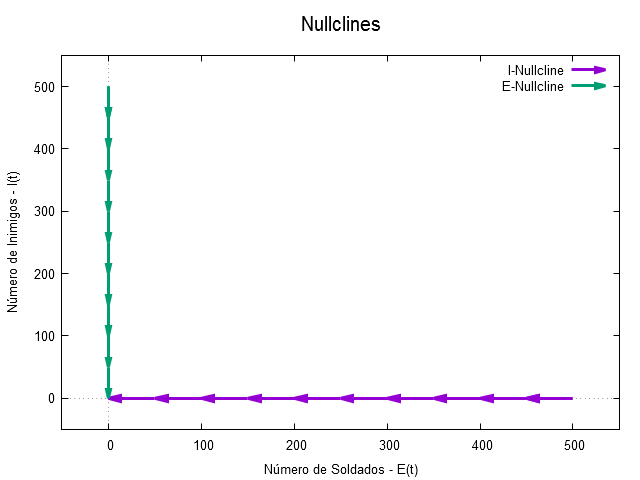
\includegraphics[scale=0.4]{figs/nullclines.png}
	\caption{Gráfico com as \textit{Nullclines} de $E(t)$ vs $I(t)$.}
	\label{fig:nullclines}
\end{figure}

\subsection{Plano de Fase}

O comportamento das soluções do modelo descritos pelo gráfico de \textit{Nullclines} é corroborado pelo plano de fase dos termos de reação do sistema. Como pode ser visto na Figura \ref{fig:phase-plane}, construída como um campo vetorial de $I(t)$ vs $E(t)$, todas as soluções são levadas para algum dos eixos canônicos.

Pela Figura também é possível perceber que a taxa com que a quantidade de soldados caí no decorrer da batalha é maior quando existem muitos soldados em campo. O que faz sentido, dado que quanto mais soldados em batalha maior a chance de acontecer um acerto por parte do adversário. A medida que o número de soldados vai caindo, a taxa com que o número de soldados caí também é reduzida. Na Figura \ref{fig:phase-plane} foi escolhido o desenho do campo vetorial no lugar do campo de direções para evidenciar esse fato.

A Figura \ref{fig:phase-plane} também é composta pela solução numérica do modelo de acordo com os dados de entrada da Tabela \ref{tb:input}. Os vetores da figura deveriam representar a direção da derivada em cada um dos pontos. Note que isso não acontece na Figura \ref{fig:phase-plane}. Esse fato é decorrente da influência do termo de difusão na solução do sistema. O número de inimigos, para essa solução particular, decresce mais rapidamente que o número de soldados do exército quando a munição fica disponível na linha de frente. Essa disponibilidade é a influência do termo de difusão na solução.

\begin{figure}[ht]
	\centering
	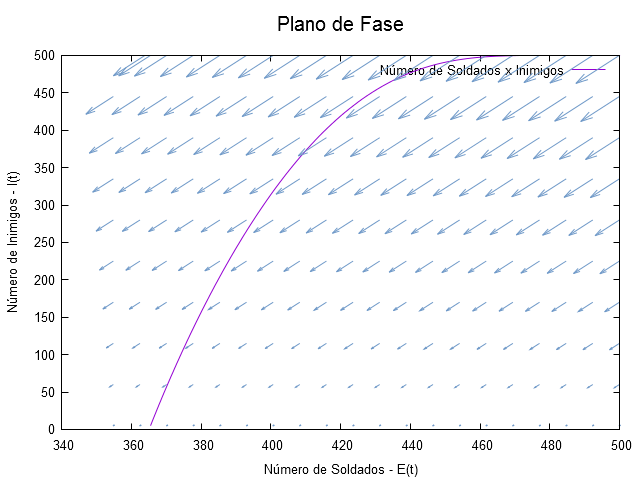
\includegraphics[scale=0.4]{figs/battle_phase_plane.png}
	\caption{Resultado da batalha para os dados de entrada da Tabela \ref{tb:input}. Nestas condições o exército sai vitorioso.}
	\label{fig:phase-plane}
\end{figure}

\section{Resultados}

\begin{figure}[ht]
	\centering
	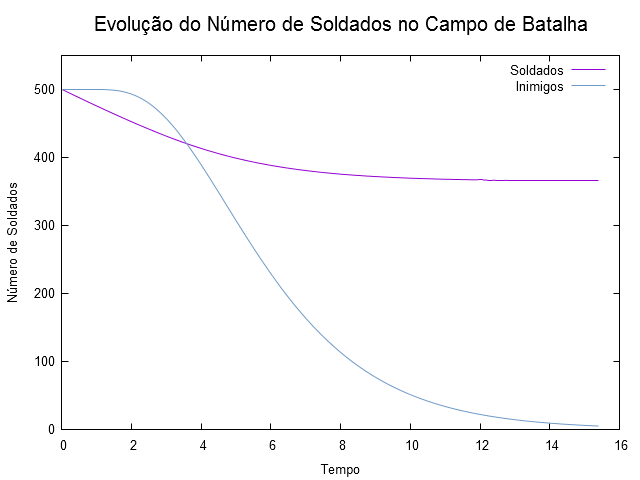
\includegraphics[scale=0.4]{figs/battle_reaction.png}
	\caption{Resultado da batalha para os dados de entrada da Tabela \ref{tb:input}. Nestas condições o exército sai vitorioso.}
	\label{fig:battle1}
\end{figure}

\begin{figure}[ht]
	\centering
	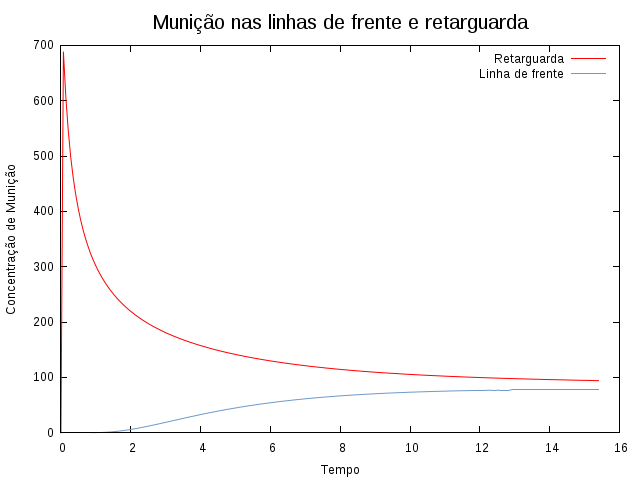
\includegraphics[scale=0.4]{figs/battle_ammo_diffusion.png}
	\caption{Difusão da munição a partir da retaguarda até a linha de frente. Como a munição se concentra totalmente na retaguarda, ela rapidamente chega a linha de frente.}
	\label{fig:battle1-ammo}
\end{figure}

A Figura \ref{fig:battle1} mostra o resultado da batalha descrita pelos dados de entrada mostrados na Tabela \ref{tb:input}. É possível ver claramente que a estratégia de manter uma formação compacta, com uma pequena quantidade de soldados na linha-de-frente, é eficiente. É possível ver claramente o momento em que a munição começa a 

A Figura \ref{fig:battle1-ammo} mostra a concentração de munição tanto na retaguarda quando na linha de frente para o exército sendo modelado. Note que, no inicio da batalha, o exército começa sofrente baixas, porém como a linha de frente é relativamente pequena em relação ao número de soldados, as baixas não representam perdas significativas do contingente de soldados. Por volta de $t = 2$, quando a munição começa a chegar na linha de frente, é possível ver uma reviravolta drástica no destino da batalha. Como a perícia e o poder de fogo do exército são maiores em relação ao inimigo, quando a munição fica disponível na linha de frente, a queda no contingente inimigo é significativa levando-os a vitória.

Pode-se argumentar que não ter munição na linha de frente é uma falha do modelo, mas nesse ponto é razoável assumir que a munição presente na linha de frente não é suficiente para causar dano no inimigo, tornando a modelagem válida.

\section{Conclusão}

Neste trabalho foi apresentado um modelo matemático que descreve a evolução de uma batalha entre duas forças homogêneas com munição limitada na linha de frente. O modelo considera que a munição que é difundida pelo exército de forma que ela deve ser levada da retaguarda para a linha de frente para que a mesma possa causar impacto no inimigo.

Fica evidente que o impacto que a munição tem ao decidir o destino da batalha é significativo. Manter uma fração do exército na linha de frente contando com substituição contínua dos soldados impacta no tempo total da batalha.

O modelo descrito, apesar de simples, pode ser utilizado para descrever o comportamento de uma batalha entre duas forças homogêneas e pode ser uma ferramenta para entender o desfecho de batalhas desse tipo que ocorriam antes dos conflitos armados modernos.

As análises de \textit{Nullclines} e Plano de Fase foram baseadas na teoria apresentada em \cite{chaos}.


%----------------------------------------------------------------------------------------
%	BIBLIOGRAPHY
%----------------------------------------------------------------------------------------

\bibliographystyle{acm}
\bibliography{references}

%----------------------------------------------------------------------------------------

\newpage
\appendix
\section{Código Fonte com a Implementação do Modelo}

\lstinputlisting{../src/main.cpp}

\end{document}
